\section{Problem Setup}

\subsection{Setting and Goal}
\label{sec:problem}

A window of a sensor stream is generated by latent factors that separate into two groups by timescale,
\begin{equation}
x_{[t-L,\,t]} \;=\; G\big(s_{[t-L,\,t]},\ u_{[t-L,\,t]}\big),
\label{eq:setting}
\end{equation}
where $s$ changes slowly and $u$ fast. Neither is observed, and neither is labelled during training. The signal is a functional of the two factor \emph{paths} rather than a mixture of their instantaneous values, because a factor may set the frequency of an oscillation instead of adding to it, in which case $x_t$ depends on the history of $s$ and not on $s_t$.

What ``slow'' and ``fast'' mean is fixed by a single timescale $\tau$: a factor is \textbf{persistent} if it still contributes to predicting the signal more than $\tau$ ahead, and \textbf{transient} otherwise. Persistence in this sense is a property of a factor relative to $\tau$ and not of the factor alone --- walking is persistent against a threshold of one second and transient against one of a day, with nothing about the factor changed. $\tau$ is a hyperparameter here, and one that cannot be set without labels (Section~\ref{sec:limits}).

\paragraph{Goal.} We want an encoder whose output carries the persistent factor, and not the transient one, at a designated subset of the embedding coordinates chosen before training. We write that subset $\zslow$ and the remaining coordinates $\zmix$. Formally: $s$ readable from $\zslow$ and $u$ not readable from $\zslow$, both under a probe class fixed in advance, which we take to be linear throughout. That the coordinates are fixed before training is part of the requirement and not a convenience: recovering them by rotating a trained embedding is a different problem. Section~\ref{sec:rotation} compares against that alternative, and measures what changes when the probe is not linear.

\paragraph{What would count as success.} Three conditions have to hold together, since each alone has a degenerate solution: the persistent factor readable from $\zslow$ (\emph{inclusion}), the transient factor readable from $\zmix$ (\emph{allocation}), and the transient factor unreadable from $\zslow$ (\emph{exclusion}). Section~\ref{sec:measure} turns them into a measurement. They are not of equal difficulty. A predictive objective is indifferent to which coordinates hold a factor, so a factor present anywhere in the embedding can be read from almost any subspace of the same width, and placing $s$ in $\zslow$ is close to free; nothing in that objective, on the other hand, pushes information \emph{out of} a subspace where it is still allowed to help. \textbf{The problem is one-sided: not to gather the persistent factor into a block, but to empty the transient one out of it.}

\subsection{Where Persistence is not Slowness}
\label{sec:synthetic}

If persistence and spectral slowness always agreed, a horizon gate would be an expensive way to reach what a low-pass filter already gives. We therefore build data in which the two disagree by construction.

\begin{figure}[!htb]
\centering
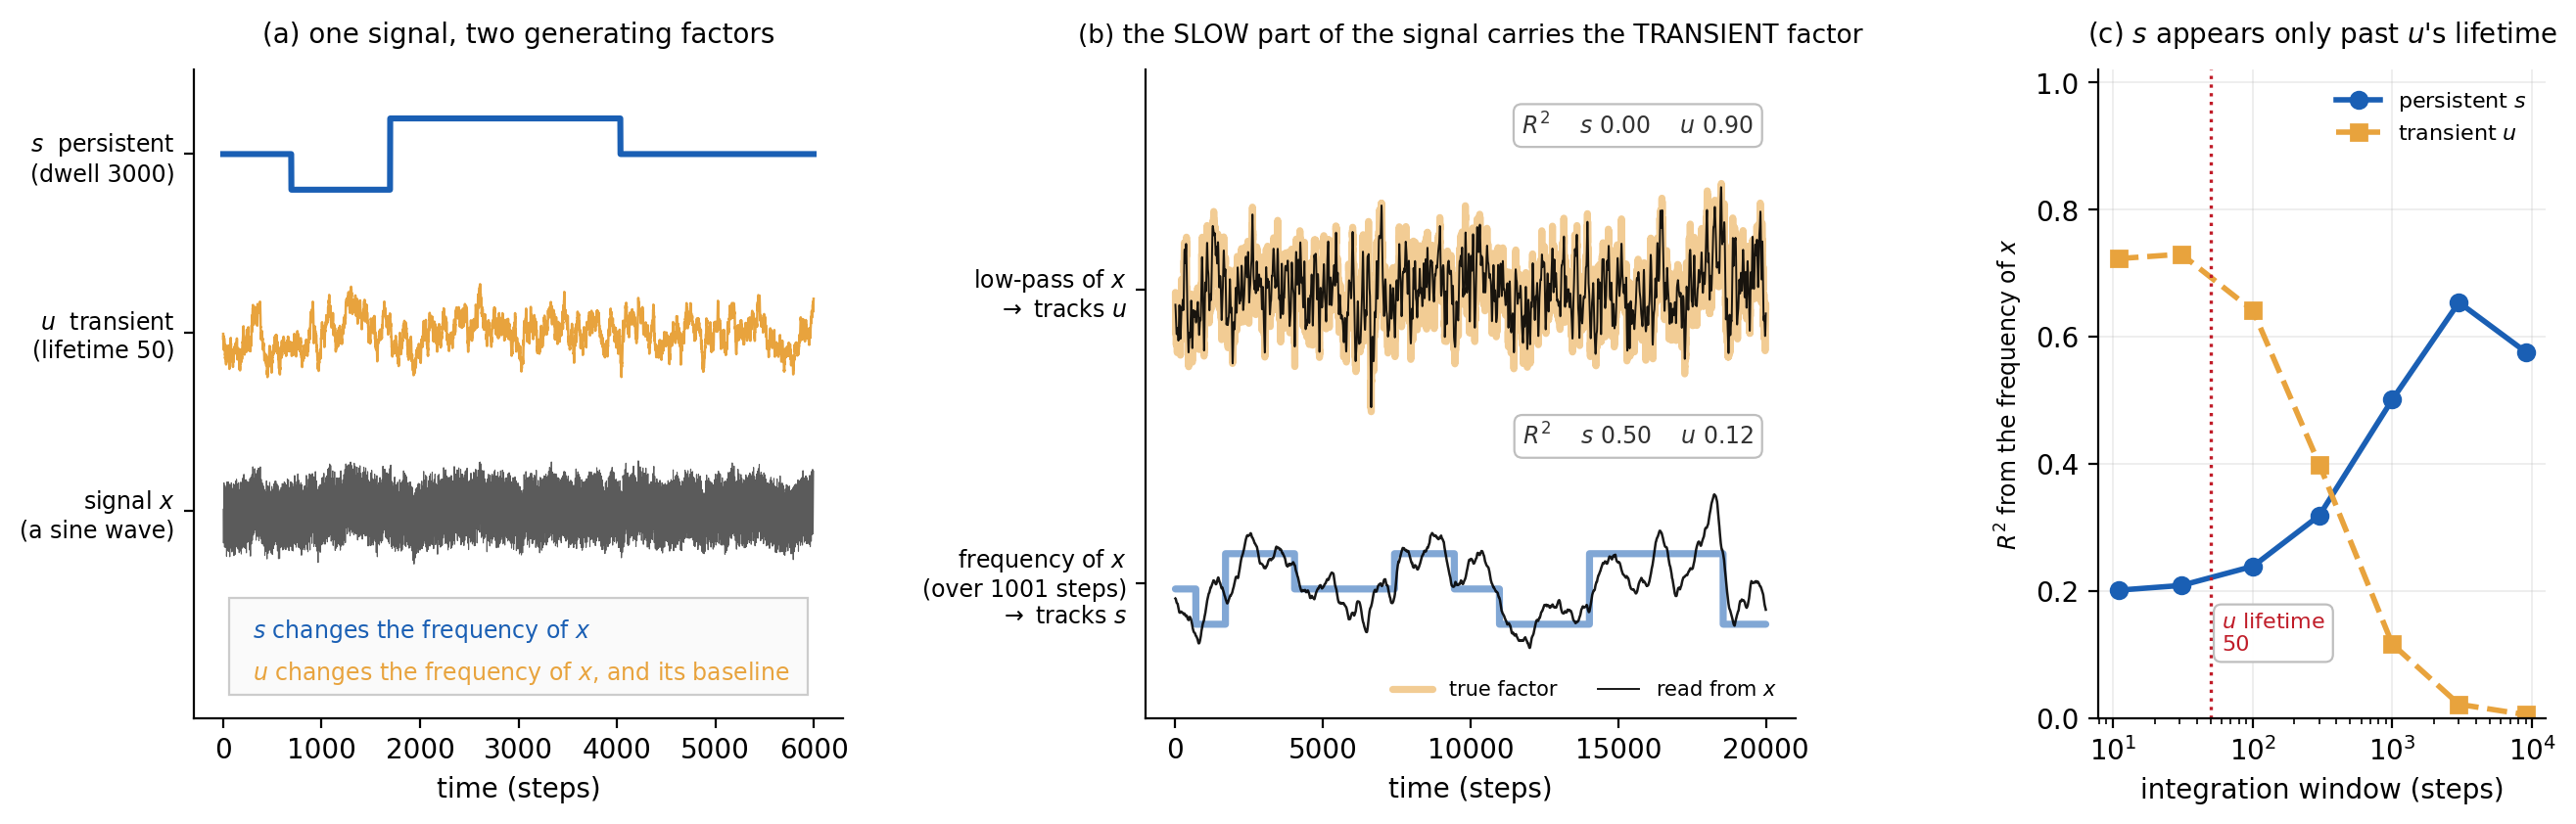
\includegraphics[width=0.94\textwidth]{figs/fig_persistence.png}
\caption{\textbf{Spectral slowness is not factor persistence.} One synthetic series, 400,000 steps, one seed. \textbf{(a)} The two factors and the signal they generate. \textbf{(b)} The slow part of $x$ against the frequency of $x$ read over a 1,001-step window, each scored on both factors. \textbf{(c)} The same $R^2$ against the width of that window.}
\label{fig:persistence}
\end{figure}

A three-state Markov persistent factor $s$ (mean dwell 3{,}000 steps) sets the carrier frequency of an oscillation, spaced $\pm$3\% around 0.100; a transient Ornstein--Uhlenbeck factor $u$ (autocorrelation time 50 steps) modulates that instantaneous frequency and adds to the signal. Amplitude is identical across regimes, so a regime change alters \emph{only how fast the signal oscillates}. The two timescales are cleanly separated --- autocorrelation half-lives 1,859 and 51 steps --- so $s$ is persistent by any reading. Yet it is absent from the slow part of the signal: a low-pass reading ($f<0.02$) recovers the \emph{transient} factor at $R^2=0.90$ and the persistent one at $R^2<10^{-5}$ (Fig.~\ref{fig:persistence}b). The persistent factor is carried by the fastest-changing part of the signal and the transient factor enters as the slower additive term, which is the exact reversal of what a slowness criterion assumes.

The persistent factor is still readable, but only through a nonlinear statistic and only over a wide enough window: the instantaneous frequency over 1,001 steps recovers it at $R^2=0.50$, and the recovery appears only once the window is tens of times $u$'s lifetime, falling away again when the window grows wide enough to blur $s$ itself (Fig.~\ref{fig:persistence}c). This is the general shape of the situation, not an artifact of our generator: while a factor persists, what stays fixed is not the signal but its statistics, and those surface only through some function of the signal.

Difficulty is set by the spacing between regime frequencies and calibrated by a training-free FFT reader, so that the task is neither trivially solved nor unsolvable before any representation is learned. At $\pm$3\% the reader reaches accuracy 0.660 (chance 0.333); at $\pm$5\% it already reaches 0.784 before any training, and at $\pm$1\% it falls to 0.459, near chance. We use $\pm$3\% throughout.

\subsection{What We Measure}
\label{sec:measure}

The three conditions become a \textbf{block $\times$ factor matrix} scoring both blocks on both factors, and a single-number summary \textbf{SEP}.

\begin{enumerate}
\item \textbf{Inclusion --- is the persistent factor in $\zslow$?} We score how well the persistent factor is predicted from $\zslow$ alone.
\item \textbf{Allocation --- is the transient factor in $\zmix$?} We score how well the transient proxy is recovered from $\zmix$ alone.
\item \textbf{Exclusion --- is the transient factor absent from $\zslow$?} We measure how well the transient proxy can be recovered from $\zslow$, and subtract that value from 1.
\end{enumerate}

\begin{equation}
\mathrm{SEP} = \underbrace{\big[s_{\text{per}}(z^{\mathrm{per}})\big]_0^1}_{\text{inclusion}} \cdot \underbrace{\big[s_{\text{tra}}(z^{\mathrm{mix}})\big]_0^1}_{\text{allocation}} \cdot \underbrace{\big[1-s_{\text{tra}}(z^{\mathrm{per}})\big]_0^1}_{\text{exclusion}}
\label{eq:sep}
\end{equation}

$s_{\text{per}}(\cdot)$ scores reading the \emph{persistent factor} from a subspace and $s_{\text{tra}}(\cdot)$ the \emph{transient proxy}; $[\cdot]_0^1$ clips into $[0,1]$. Classification scores already lie in this range, but $R^2$ goes negative when a prediction is worse than the mean, and the clipping acts only there, preventing a negative value from flipping the sign of the product. There is no normalization by any denominator anywhere.
